
\begin{figure*}[t]
	\newcommand{\CreateGradientColorCell}[3]{%
		\ifdim #1 pt > \MidNumber pt
			\pgfmathsetmacro{\PercentColor}{max(min(100.0*(#1 - \MidNumber)/(\MaxNumber-\MidNumber),100.0),0.00)} %
			\node[draw=#3, Node, fill=\MaxColor!\PercentColor!\MidColor] at #2 {\scalebox{0.5}{#1}};
		\else
			\pgfmathsetmacro{\PercentColor}{max(min(100.0*(\MidNumber - #1)/(\MidNumber-\MinNumber),100.0),0.00)} %
			\node[draw=#3, Node, fill=\MinColor!\PercentColor!\MidColor] at #2 {\scalebox{0.5}{#1}};
		\fi
	}
	\newcommand{\CreateGradientColorCellWithName}[5]{%
		\ifdim #1 pt > \MidNumber pt
			\pgfmathsetmacro{\PercentColor}{max(min(100.0*(#1 - \MidNumber)/(\MaxNumber-\MidNumber),100.0),0.00)} %
			\node[draw=#3, #5, fill=\MaxColor!\PercentColor!\MidColor] at #2 {\setstretch{0.8}\scalebox{0.6}{#4}\\\scalebox{0.6}{#1}};
		\else
			\pgfmathsetmacro{\PercentColor}{max(min(100.0*(\MidNumber - #1)/(\MidNumber-\MinNumber),100.0),0.00)} %
			\node[draw=#3, #5, fill=\MinColor!\PercentColor!\MidColor] at #2 {\setstretch{0.8}\scalebox{0.6}{#4}\\\scalebox{0.6}{#1}};
		\fi
	}
	\newcommand{\CreateLogTwoGradientColorCell}[3]{%
		\ifdim #1 pt > \MidNumber pt
			\pgfmathsetmacro{\PercentColor}{max(min(100.0*(#1 - \MidNumber)/(\MaxNumber-\MidNumber),100.0),0.00)} %
			\node[draw=#3, Node, fill=\MaxColor!\PercentColor!\MidColor] at #2 {\scalebox{0.5}{$2^{#1}$}};
		\else
			\pgfmathsetmacro{\PercentColor}{max(min(100.0*(\MidNumber - #1)/(\MidNumber-\MinNumber),100.0),0.00)} %
			\node[draw=#3, Node, fill=\MinColor!\PercentColor!\MidColor] at #2 {\scalebox{0.5}{$2^{#1}$}};
		\fi
	}
	\centering
	\newcommand*{\HighlighColor}{black}
	\newcommand*{\MaxNumber}{1.313}
	\newcommand*{\MidNumber}{1}
	\newcommand*{\MinNumber}{0.965}
	\newcommand*{\MaxColor}{red}
	\newcommand*{\MidColor}{white}
	\newcommand*{\MinColor}{maxGreen}
	\newcommand*{\baseX}{0}
	\newcommand*{\baseY}{0}
	\newcommand*{\MinWidth}{0.5}
	\begin{subfigure}[b]{0.245\linewidth}
		\centering
		\begin{tikzpicture}[
			Node/.style = {minimum width=\MinWidth cm, minimum height=\MinWidth cm, inner sep=0,outer sep=0},
		]
			\node[Node] at (\baseX + 0 * \MinWidth,\baseY + \MinWidth) {\scalebox{\MinWidth}{128}};
			\node[Node] at (\baseX + 1 * \MinWidth,\baseY + \MinWidth) {\scalebox{\MinWidth}{256}};
			\node[Node] at (\baseX + 2 * \MinWidth,\baseY + \MinWidth) {\scalebox{\MinWidth}{512}};
			\node[Node] at (\baseX + 3 * \MinWidth,\baseY + \MinWidth) {\scalebox{\MinWidth}{1024}};
			\node[Node] at (\baseX + 4 * \MinWidth,\baseY + \MinWidth) {\scalebox{\MinWidth}{2048}};
			\node[Node] at (\baseX + 5 * \MinWidth,\baseY + \MinWidth) {\scalebox{\MinWidth}{4096}};
			\node[Node] at (\baseX + 6 * \MinWidth,\baseY + \MinWidth) {\scalebox{\MinWidth}{8192}};
			\node[Node] at (\baseX - \MinWidth,\baseY - 0 * \MinWidth) {\scalebox{\MinWidth}{128}};
			\node[Node] at (\baseX - \MinWidth,\baseY - 1 * \MinWidth) {\scalebox{\MinWidth}{256}};
			\node[Node] at (\baseX - \MinWidth,\baseY - 2 * \MinWidth) {\scalebox{\MinWidth}{512}};
			\node[Node] at (\baseX - \MinWidth,\baseY - 3 * \MinWidth) {\scalebox{\MinWidth}{1024}};
			\node[Node] at (\baseX - \MinWidth,\baseY - 4 * \MinWidth) {\scalebox{\MinWidth}{2048}};
			\node[Node] at (\baseX - \MinWidth,\baseY - 5 * \MinWidth) {\scalebox{\MinWidth}{4096}};
			\node[Node] at (\baseX - \MinWidth,\baseY - 6 * \MinWidth) {\scalebox{\MinWidth}{8192}};
			\renewcommand{\baseY}{-1 * 0 * \MinWidth}%
			\CreateGradientColorCell{0.988}{(\baseX + 0 * \MinWidth,\baseY - 0.0)}{none}
			\CreateGradientColorCell{0.984}{(\baseX + 1 * \MinWidth,\baseY - 0.0)}{none}
			\CreateGradientColorCell{0.980}{(\baseX + 2 * \MinWidth,\baseY - 0.0)}{none}
			\CreateGradientColorCell{0.973}{(\baseX + 3 * \MinWidth,\baseY - 0.0)}{none}
			\CreateGradientColorCell{0.970}{(\baseX + 4 * \MinWidth,\baseY - 0.0)}{none}
			\CreateGradientColorCell{0.967}{(\baseX + 5 * \MinWidth,\baseY - 0.0)}{none}
			\CreateGradientColorCell{0.966}{(\baseX + 6 * \MinWidth,\baseY - 0.0)}{none}
			\renewcommand{\baseY}{-1 * 1 * \MinWidth}%
			\CreateGradientColorCell{0.980}{(\baseX + 0 * \MinWidth,\baseY - 0.0)}{none}
			\CreateGradientColorCell{0.979}{(\baseX + 1 * \MinWidth,\baseY - 0.0)}{none}
			\CreateGradientColorCell{0.974}{(\baseX + 2 * \MinWidth,\baseY - 0.0)}{none}
			\CreateGradientColorCell{0.970}{(\baseX + 3 * \MinWidth,\baseY - 0.0)}{none}
			\CreateGradientColorCell{0.968}{(\baseX + 4 * \MinWidth,\baseY - 0.0)}{none}
			\CreateGradientColorCell{0.966}{(\baseX + 5 * \MinWidth,\baseY - 0.0)}{none}
			\CreateGradientColorCell{0.966}{(\baseX + 6 * \MinWidth,\baseY - 0.0)}{none}
			\renewcommand{\baseY}{-1 * 2 * \MinWidth}%
			\CreateGradientColorCell{0.980}{(\baseX + 0 * \MinWidth,\baseY - 0.0)}{none}
			\CreateGradientColorCell{0.974}{(\baseX + 1 * \MinWidth,\baseY - 0.0)}{none}
			\CreateGradientColorCell{0.971}{(\baseX + 2 * \MinWidth,\baseY - 0.0)}{none}
			\CreateGradientColorCell{0.968}{(\baseX + 3 * \MinWidth,\baseY - 0.0)}{none}
			\CreateGradientColorCell{0.966}{(\baseX + 4 * \MinWidth,\baseY - 0.0)}{none}
			\CreateGradientColorCell{0.966}{(\baseX + 5 * \MinWidth,\baseY - 0.0)}{none}
			\CreateGradientColorCell{0.965}{(\baseX + 6 * \MinWidth,\baseY - 0.0)}{none}
			\renewcommand{\baseY}{-1 * 3 * \MinWidth}%
			\CreateGradientColorCell{0.976}{(\baseX + 0 * \MinWidth,\baseY - 0.0)}{none}
			\CreateGradientColorCell{0.971}{(\baseX + 1 * \MinWidth,\baseY - 0.0)}{none}
			\CreateGradientColorCell{0.969}{(\baseX + 2 * \MinWidth,\baseY - 0.0)}{none}
			\CreateGradientColorCell{0.967}{(\baseX + 3 * \MinWidth,\baseY - 0.0)}{none}
			\CreateGradientColorCell{0.966}{(\baseX + 4 * \MinWidth,\baseY - 0.0)}{none}
			\CreateGradientColorCell{0.966}{(\baseX + 5 * \MinWidth,\baseY - 0.0)}{none}
			\CreateGradientColorCell{0.965}{(\baseX + 6 * \MinWidth,\baseY - 0.0)}{none}
			\renewcommand{\baseY}{-1 * 4 * \MinWidth}%
			\CreateGradientColorCell{0.973}{(\baseX + 0 * \MinWidth,\baseY - 0.0)}{none}
			\CreateGradientColorCell{0.969}{(\baseX + 1 * \MinWidth,\baseY - 0.0)}{none}
			\CreateGradientColorCell{0.967}{(\baseX + 2 * \MinWidth,\baseY - 0.0)}{none}
			\CreateGradientColorCell{0.966}{(\baseX + 3 * \MinWidth,\baseY - 0.0)}{none}
			\CreateGradientColorCell{0.966}{(\baseX + 4 * \MinWidth,\baseY - 0.0)}{none}
			\CreateGradientColorCell{0.965}{(\baseX + 5 * \MinWidth,\baseY - 0.0)}{none}
			\CreateGradientColorCell{0.965}{(\baseX + 6 * \MinWidth,\baseY - 0.0)}{none}
			\renewcommand{\baseY}{-1 * 5 * \MinWidth}%
			\CreateGradientColorCell{0.971}{(\baseX + 0 * \MinWidth,\baseY - 0.0)}{none}
			\CreateGradientColorCell{0.968}{(\baseX + 1 * \MinWidth,\baseY - 0.0)}{none}
			\CreateGradientColorCell{0.967}{(\baseX + 2 * \MinWidth,\baseY - 0.0)}{none}
			\CreateGradientColorCell{0.966}{(\baseX + 3 * \MinWidth,\baseY - 0.0)}{none}
			\CreateGradientColorCell{0.966}{(\baseX + 4 * \MinWidth,\baseY - 0.0)}{none}
			\CreateGradientColorCell{0.965}{(\baseX + 5 * \MinWidth,\baseY - 0.0)}{none}
			\CreateGradientColorCell{0.965}{(\baseX + 6 * \MinWidth,\baseY - 0.0)}{none}
			\renewcommand{\baseY}{-1 * 6 * \MinWidth}%
			\CreateGradientColorCell{0.970}{(\baseX + 0 * \MinWidth,\baseY - 0.0)}{none}
			\CreateGradientColorCell{0.968}{(\baseX + 1 * \MinWidth,\baseY - 0.0)}{none}
			\CreateGradientColorCell{0.966}{(\baseX + 2 * \MinWidth,\baseY - 0.0)}{none}
			\CreateGradientColorCell{0.966}{(\baseX + 3 * \MinWidth,\baseY - 0.0)}{none}
			\CreateGradientColorCell{0.965}{(\baseX + 4 * \MinWidth,\baseY - 0.0)}{none}
			\CreateGradientColorCell{0.965}{(\baseX + 5 * \MinWidth,\baseY - 0.0)}{\HighlighColor}
			\CreateGradientColorCell{0.965}{(\baseX + 6 * \MinWidth,\baseY - 0.0)}{none}

			\draw[->] (-1 * \MinWidth / 2,\MinWidth / 2) -- (\MinWidth * 7 - \MinWidth / 2,\MinWidth / 2);
			\node[minimum height=\MinWidth cm, inner sep=0,outer sep=0] at (\MinWidth * 7 / 2 - \MinWidth / 2,0.75) {\scalebox{\MinWidth}{Input Size}};
			\draw[->] (-1 * \MinWidth / 2,\MinWidth / 2) -- (-1 * \MinWidth / 2,-1 * \MinWidth * 7 + \MinWidth / 2);
			\node[minimum height=\MinWidth cm, inner sep=0,outer sep=0] at (-0.2,-1 * \MinWidth * 7) {\scalebox{\MinWidth}{Output Size}};
		\end{tikzpicture}
		\caption{
			\centering
			\ourmethod{} for $W2A2$
		}
		\label{fig:appendix:instructions:w2a2}
	\end{subfigure}
	\begin{subfigure}[b]{0.245\linewidth}
		\centering
		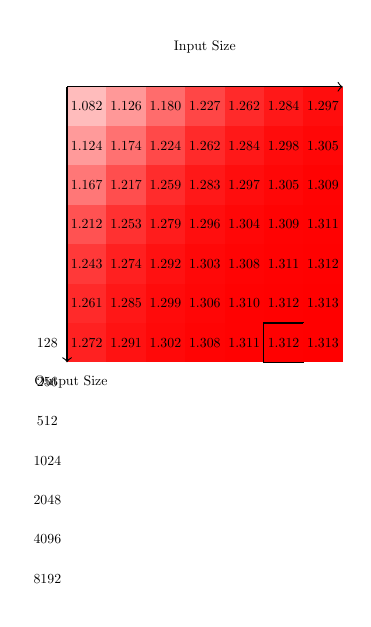
\begin{tikzpicture}[
			Node/.style = {minimum width=\MinWidth cm, minimum height=\MinWidth cm, inner sep=0,outer sep=0},
		]
			\node[Node] at (\baseX + 0 * \MinWidth,\baseY + \MinWidth) {\scalebox{\MinWidth}{128}};
			\node[Node] at (\baseX + 1 * \MinWidth,\baseY + \MinWidth) {\scalebox{\MinWidth}{256}};
			\node[Node] at (\baseX + 2 * \MinWidth,\baseY + \MinWidth) {\scalebox{\MinWidth}{512}};
			\node[Node] at (\baseX + 3 * \MinWidth,\baseY + \MinWidth) {\scalebox{\MinWidth}{1024}};
			\node[Node] at (\baseX + 4 * \MinWidth,\baseY + \MinWidth) {\scalebox{\MinWidth}{2048}};
			\node[Node] at (\baseX + 5 * \MinWidth,\baseY + \MinWidth) {\scalebox{\MinWidth}{4096}};
			\node[Node] at (\baseX + 6 * \MinWidth,\baseY + \MinWidth) {\scalebox{\MinWidth}{8192}};
			\node[Node] at (\baseX - \MinWidth,\baseY - 0 * \MinWidth) {\scalebox{\MinWidth}{128}};
			\node[Node] at (\baseX - \MinWidth,\baseY - 1 * \MinWidth) {\scalebox{\MinWidth}{256}};
			\node[Node] at (\baseX - \MinWidth,\baseY - 2 * \MinWidth) {\scalebox{\MinWidth}{512}};
			\node[Node] at (\baseX - \MinWidth,\baseY - 3 * \MinWidth) {\scalebox{\MinWidth}{1024}};
			\node[Node] at (\baseX - \MinWidth,\baseY - 4 * \MinWidth) {\scalebox{\MinWidth}{2048}};
			\node[Node] at (\baseX - \MinWidth,\baseY - 5 * \MinWidth) {\scalebox{\MinWidth}{4096}};
			\node[Node] at (\baseX - \MinWidth,\baseY - 6 * \MinWidth) {\scalebox{\MinWidth}{8192}};
			\renewcommand{\baseY}{-1 * 0 * \MinWidth}%
			\CreateGradientColorCell{1.082}{(\baseX + 0 * \MinWidth,\baseY - 0.0)}{none}
			\CreateGradientColorCell{1.126}{(\baseX + 1 * \MinWidth,\baseY - 0.0)}{none}
			\CreateGradientColorCell{1.180}{(\baseX + 2 * \MinWidth,\baseY - 0.0)}{none}
			\CreateGradientColorCell{1.227}{(\baseX + 3 * \MinWidth,\baseY - 0.0)}{none}
			\CreateGradientColorCell{1.262}{(\baseX + 4 * \MinWidth,\baseY - 0.0)}{none}
			\CreateGradientColorCell{1.284}{(\baseX + 5 * \MinWidth,\baseY - 0.0)}{none}
			\CreateGradientColorCell{1.297}{(\baseX + 6 * \MinWidth,\baseY - 0.0)}{none}
			\renewcommand{\baseY}{-1 * 1 * \MinWidth}%
			\CreateGradientColorCell{1.124}{(\baseX + 0 * \MinWidth,\baseY - 0.0)}{none}
			\CreateGradientColorCell{1.174}{(\baseX + 1 * \MinWidth,\baseY - 0.0)}{none}
			\CreateGradientColorCell{1.224}{(\baseX + 2 * \MinWidth,\baseY - 0.0)}{none}
			\CreateGradientColorCell{1.262}{(\baseX + 3 * \MinWidth,\baseY - 0.0)}{none}
			\CreateGradientColorCell{1.284}{(\baseX + 4 * \MinWidth,\baseY - 0.0)}{none}
			\CreateGradientColorCell{1.298}{(\baseX + 5 * \MinWidth,\baseY - 0.0)}{none}
			\CreateGradientColorCell{1.305}{(\baseX + 6 * \MinWidth,\baseY - 0.0)}{none}
			\renewcommand{\baseY}{-1 * 2 * \MinWidth}%
			\CreateGradientColorCell{1.167}{(\baseX + 0 * \MinWidth,\baseY - 0.0)}{none}
			\CreateGradientColorCell{1.217}{(\baseX + 1 * \MinWidth,\baseY - 0.0)}{none}
			\CreateGradientColorCell{1.259}{(\baseX + 2 * \MinWidth,\baseY - 0.0)}{none}
			\CreateGradientColorCell{1.283}{(\baseX + 3 * \MinWidth,\baseY - 0.0)}{none}
			\CreateGradientColorCell{1.297}{(\baseX + 4 * \MinWidth,\baseY - 0.0)}{none}
			\CreateGradientColorCell{1.305}{(\baseX + 5 * \MinWidth,\baseY - 0.0)}{none}
			\CreateGradientColorCell{1.309}{(\baseX + 6 * \MinWidth,\baseY - 0.0)}{none}
			\renewcommand{\baseY}{-1 * 3 * \MinWidth}%
			\CreateGradientColorCell{1.212}{(\baseX + 0 * \MinWidth,\baseY - 0.0)}{none}
			\CreateGradientColorCell{1.253}{(\baseX + 1 * \MinWidth,\baseY - 0.0)}{none}
			\CreateGradientColorCell{1.279}{(\baseX + 2 * \MinWidth,\baseY - 0.0)}{none}
			\CreateGradientColorCell{1.296}{(\baseX + 3 * \MinWidth,\baseY - 0.0)}{none}
			\CreateGradientColorCell{1.304}{(\baseX + 4 * \MinWidth,\baseY - 0.0)}{none}
			\CreateGradientColorCell{1.309}{(\baseX + 5 * \MinWidth,\baseY - 0.0)}{none}
			\CreateGradientColorCell{1.311}{(\baseX + 6 * \MinWidth,\baseY - 0.0)}{none}
			\renewcommand{\baseY}{-1 * 4 * \MinWidth}%
			\CreateGradientColorCell{1.243}{(\baseX + 0 * \MinWidth,\baseY - 0.0)}{none}
			\CreateGradientColorCell{1.274}{(\baseX + 1 * \MinWidth,\baseY - 0.0)}{none}
			\CreateGradientColorCell{1.292}{(\baseX + 2 * \MinWidth,\baseY - 0.0)}{none}
			\CreateGradientColorCell{1.303}{(\baseX + 3 * \MinWidth,\baseY - 0.0)}{none}
			\CreateGradientColorCell{1.308}{(\baseX + 4 * \MinWidth,\baseY - 0.0)}{none}
			\CreateGradientColorCell{1.311}{(\baseX + 5 * \MinWidth,\baseY - 0.0)}{none}
			\CreateGradientColorCell{1.312}{(\baseX + 6 * \MinWidth,\baseY - 0.0)}{none}
			\renewcommand{\baseY}{-1 * 5 * \MinWidth}%
			\CreateGradientColorCell{1.261}{(\baseX + 0 * \MinWidth,\baseY - 0.0)}{none}
			\CreateGradientColorCell{1.285}{(\baseX + 1 * \MinWidth,\baseY - 0.0)}{none}
			\CreateGradientColorCell{1.299}{(\baseX + 2 * \MinWidth,\baseY - 0.0)}{none}
			\CreateGradientColorCell{1.306}{(\baseX + 3 * \MinWidth,\baseY - 0.0)}{none}
			\CreateGradientColorCell{1.310}{(\baseX + 4 * \MinWidth,\baseY - 0.0)}{none}
			\CreateGradientColorCell{1.312}{(\baseX + 5 * \MinWidth,\baseY - 0.0)}{none}
			\CreateGradientColorCell{1.313}{(\baseX + 6 * \MinWidth,\baseY - 0.0)}{none}
			\renewcommand{\baseY}{-1 * 6 * \MinWidth}%
			\CreateGradientColorCell{1.272}{(\baseX + 0 * \MinWidth,\baseY - 0.0)}{none}
			\CreateGradientColorCell{1.291}{(\baseX + 1 * \MinWidth,\baseY - 0.0)}{none}
			\CreateGradientColorCell{1.302}{(\baseX + 2 * \MinWidth,\baseY - 0.0)}{none}
			\CreateGradientColorCell{1.308}{(\baseX + 3 * \MinWidth,\baseY - 0.0)}{none}
			\CreateGradientColorCell{1.311}{(\baseX + 4 * \MinWidth,\baseY - 0.0)}{none}
			\CreateGradientColorCell{1.312}{(\baseX + 5 * \MinWidth,\baseY - 0.0)}{\HighlighColor}
			\CreateGradientColorCell{1.313}{(\baseX + 6 * \MinWidth,\baseY - 0.0)}{none}

			\draw[->] (-1 * \MinWidth / 2,\MinWidth / 2) -- (\MinWidth * 7 - \MinWidth / 2,\MinWidth / 2);
			\node[minimum height=\MinWidth cm, inner sep=0,outer sep=0] at (\MinWidth * 7 / 2 - \MinWidth / 2,0.75) {\scalebox{\MinWidth}{Input Size}};
			\draw[->] (-1 * \MinWidth / 2,\MinWidth / 2) -- (-1 * \MinWidth / 2,-1 * \MinWidth * 7 + \MinWidth / 2);
			\node[minimum height=\MinWidth cm, inner sep=0,outer sep=0] at (-0.2,-1 * \MinWidth * 7) {\scalebox{\MinWidth}{Output Size}};
		\end{tikzpicture}
		\caption{
			\centering
			\ourmethod{} for $W1A1$
		}
		\label{fig:appendix:instructions:w1a1}
	\end{subfigure}
	\caption{
		\centering
		no caption 
	}
	\label{fig:appendix:instructions:mainFig}
\end{figure*}
